%
% Documento: Fundamentação Teorica
%

%\vspace{3cm}%Espaçamento entre linhas

\chapter{\textbf{DESCRIÇÃO DA SOLUÇÃO}}\label{chap:descSolucao}

Visando atender o objetivo deste trabalho de desenvolver um sistema capaz de gerenciar animais, uma solução web foi implmentada. Este capítulo detalha o desenvolvimento dessa solução, partindo do modelo de requisitos do mesmo.

A análise de requisitos do presente trabalho foi realizada através de conversas com os pecuáristas do estudo de caso. Para delimitar as funcionalidades foi elaborado um diagrama de casos de uso contendo as mesmas.

\section{MODELO DE REQUISITOS}

\begin{figure}[H]
	\begin{center}
		\caption{Diagrama de Casos de Uso do sistema}
		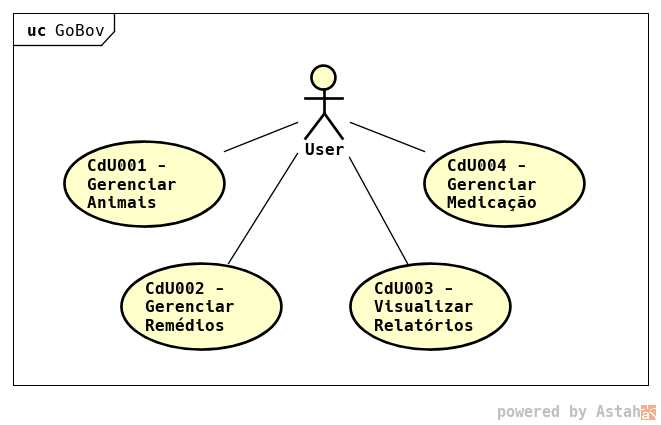
\includegraphics[width=\textwidth]{../img/casosdeuso.png}

		Fonte: Autoria própria.
	\end{center}
\end{figure}

O caso de uso Gerenciar Animal trata-se das operações realizadas com os animais, no caso, criar um animal, ler as informações dele, atualizar suas informações e deleta-lo. Os casos de uso Gerenciar Remédios e Gerenciar Medicações se referem as mesmas operações, porém, com seus respectivos objetos. O caso de uso Visualizar Relatórios se refere a visualização das informações disponibilizadas pelo sistema, aqui chamados de relatórios.


\subsection{PROTÓTIPOS DE TELA}

\begin{itemize}
\item IV001

A figura 5 é a tela de login do sistema. Nela, o usuário pode se autenticar ou se registrar.
\begin{figure}[H]
	\begin{center}
		\caption{Login no sistema}
		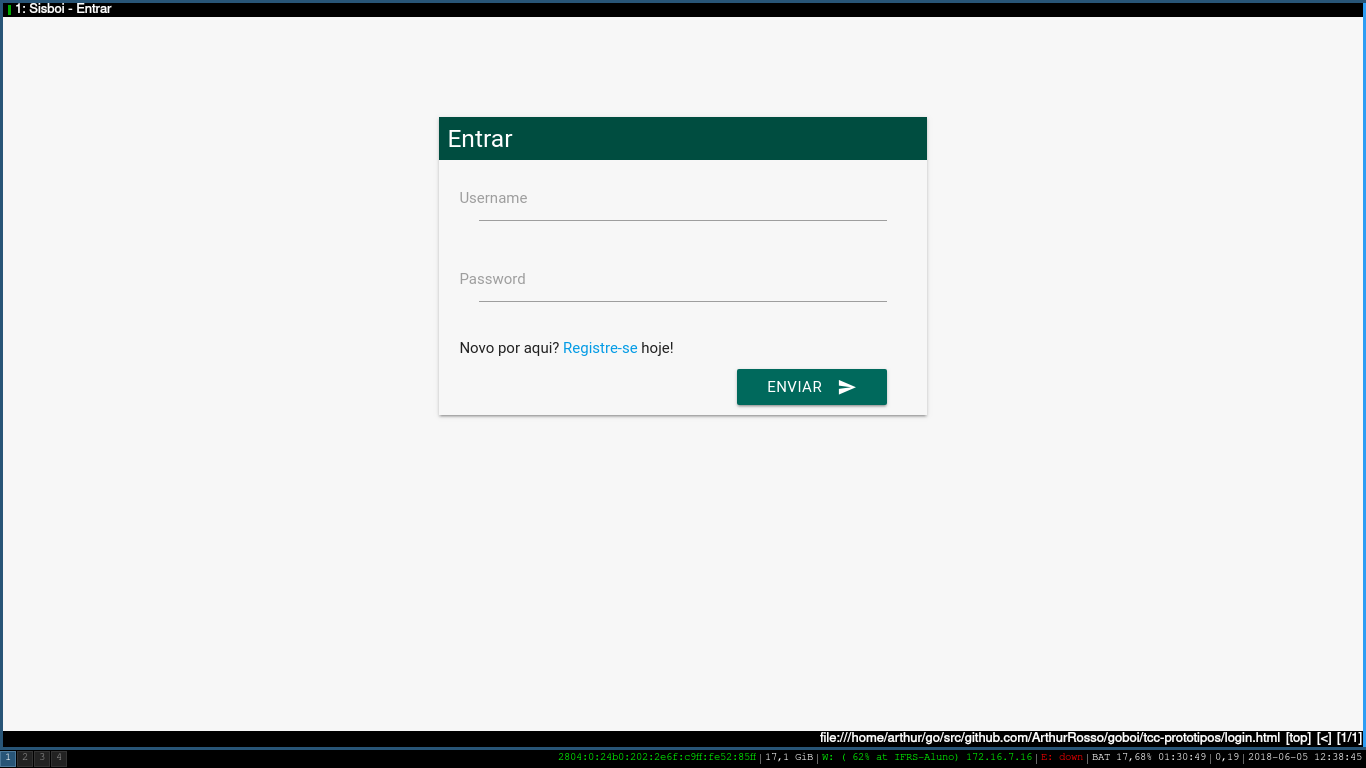
\includegraphics[width=\textwidth]{../img/prototipos/login.png}

		Fonte: Autoria própria.
	\end{center}
\end{figure}

\item IV002

A figura 6 é a tela inicial do sistema. Nela, o usuário pode ir para a tela de lista de animais, lista de Remédios, ou lista de medicações.
\begin{figure}[H]
	\begin{center}
		\caption{Página inicial do sistema}
		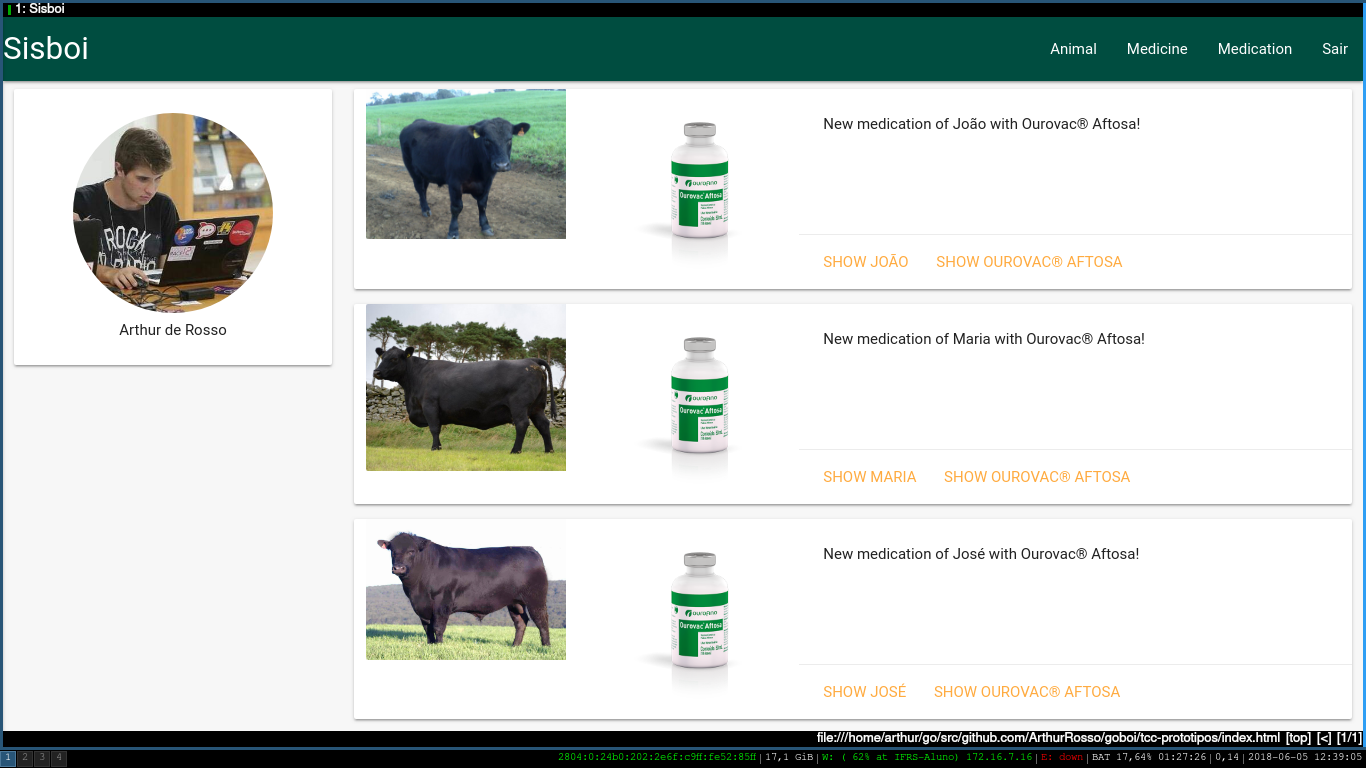
\includegraphics[width=\textwidth]{../img/prototipos/index.png}

		Fonte: Autoria própria.
	\end{center}
\end{figure}

\item IV003

A figura 7 é a página de lista de animais. Nela, o usuário pode adicionar um animal, adicionar uma medicação a um animal, pesar um animal, deletar um animal ou ir para a tela de perfil do animal.
\begin{figure}[H]
	\begin{center}
		\caption{Página do animais}
		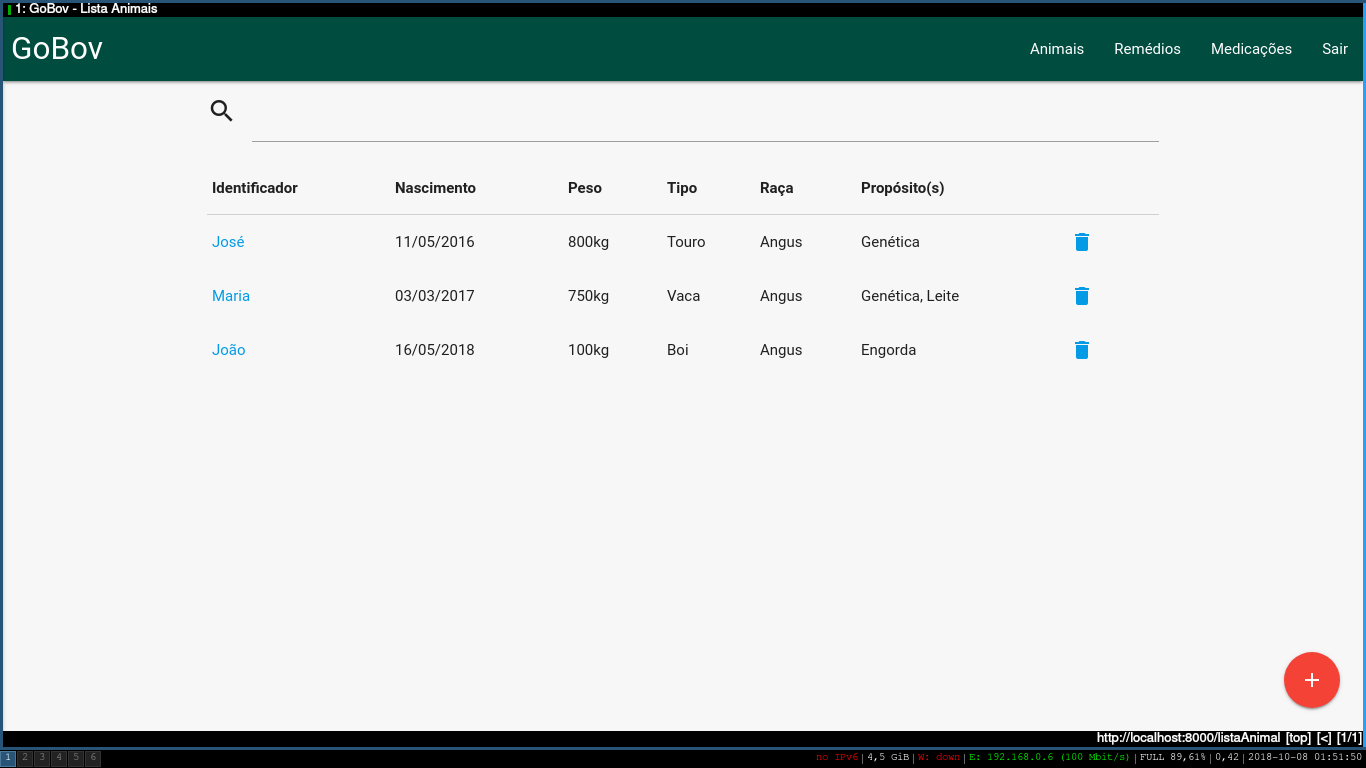
\includegraphics[width=\textwidth]{../img/prototipos/listaAnimal.png}

		Fonte: Autoria própria.
	\end{center}
\end{figure}

\item IV004

A figura 8 é a página de adicionar animal.
\begin{figure}[H]
	\begin{center}
		\caption{Página de adicionar animal}
		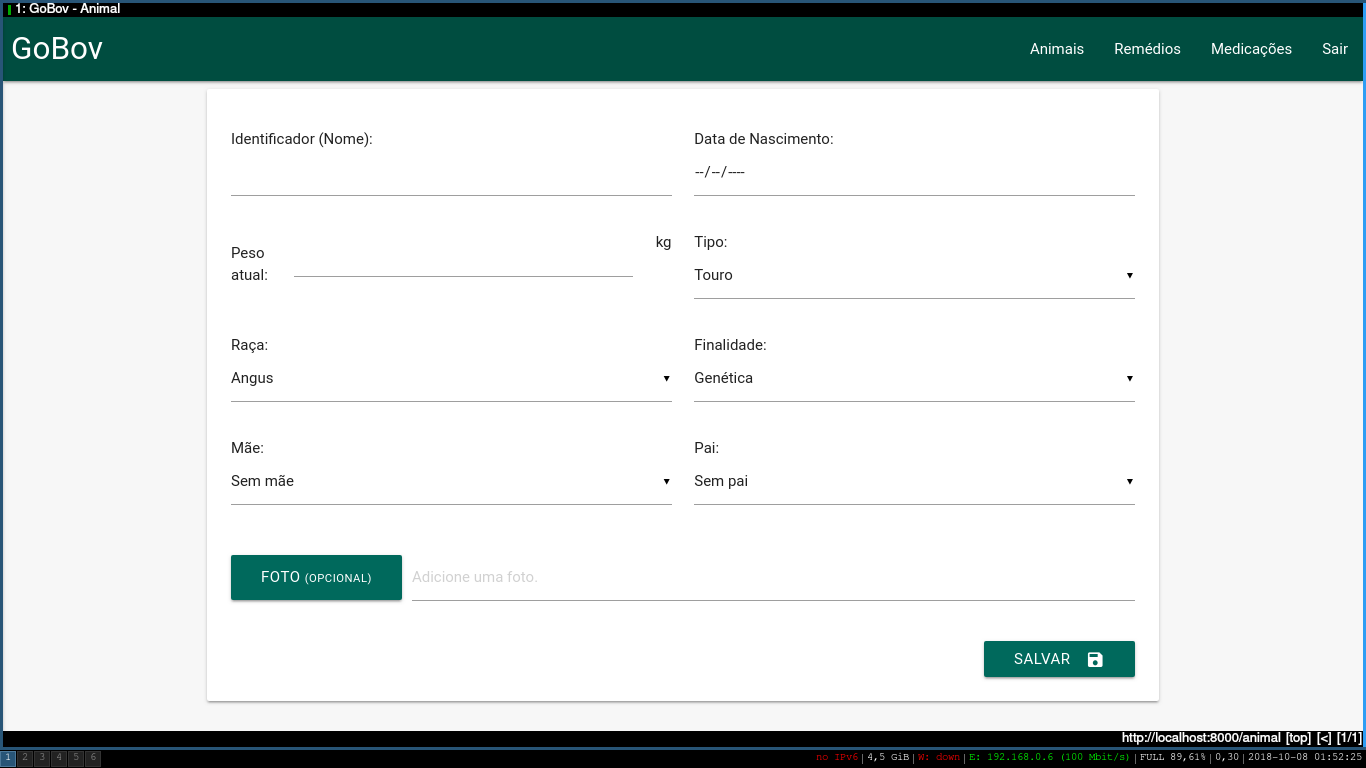
\includegraphics[width=\textwidth]{../img/prototipos/addAnimal.png}

		Fonte: Autoria própria.
	\end{center}
\end{figure}


\item IV005

A figura 9 é a página de lista de remédios. Nela, o usuário pode adicionar, deletar ou editar um remédio.
\begin{figure}[H]
	\begin{center}
		\caption{Página de remédios}
		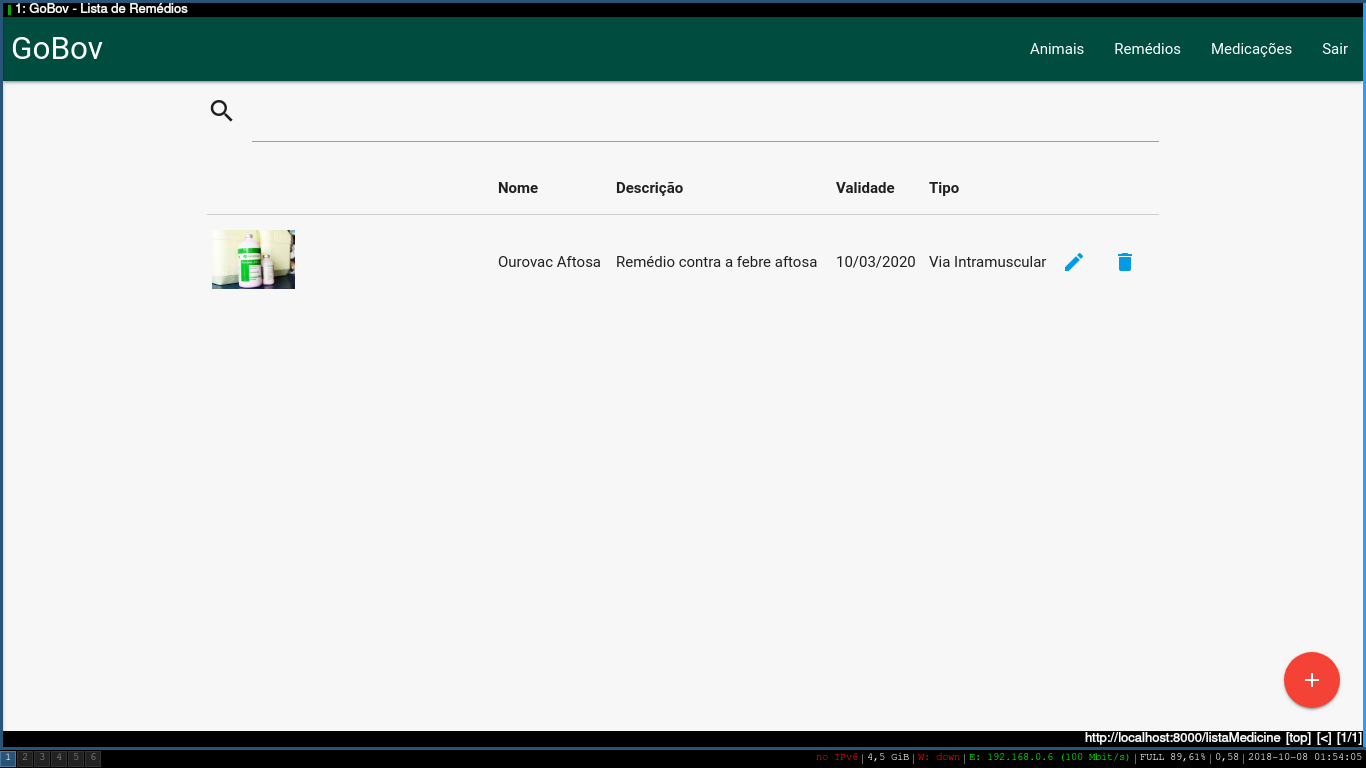
\includegraphics[width=\textwidth]{../img/prototipos/listaRemedio.png}

		Fonte: Autoria própria.
	\end{center}
\end{figure}

\item IV006

A figura 10 é a página de adicionar remédio.
\begin{figure}[H]
	\begin{center}
		\caption{Página de adicionar remédio}
		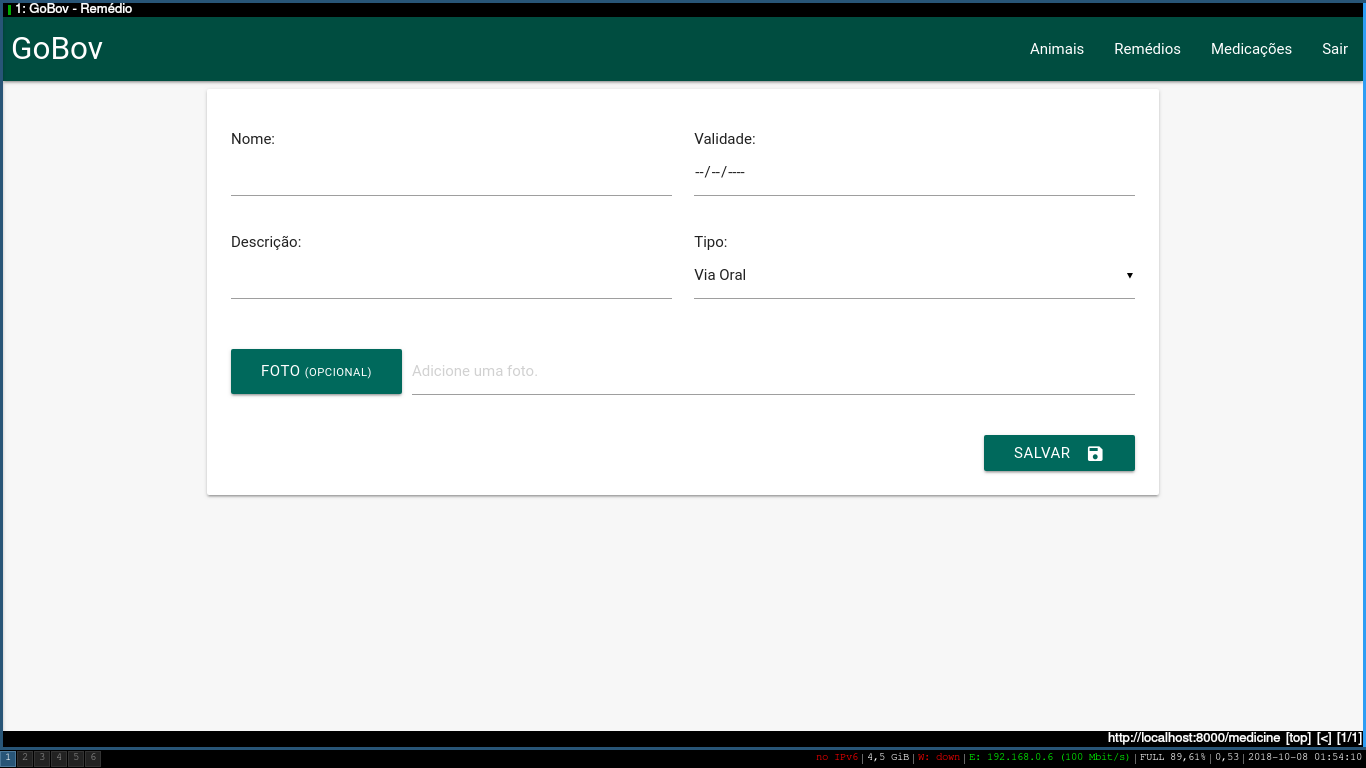
\includegraphics[width=\textwidth]{../img/prototipos/addRemedio.png}

		Fonte: Autoria própria.
	\end{center}
\end{figure}


\item IV007

A figura 11 é a página de lista de medicações. Nela, o usuário pode adicionar ou deletar uma medicação.
\begin{figure}[H]
	\begin{center}
		\caption{Página de medicações}
		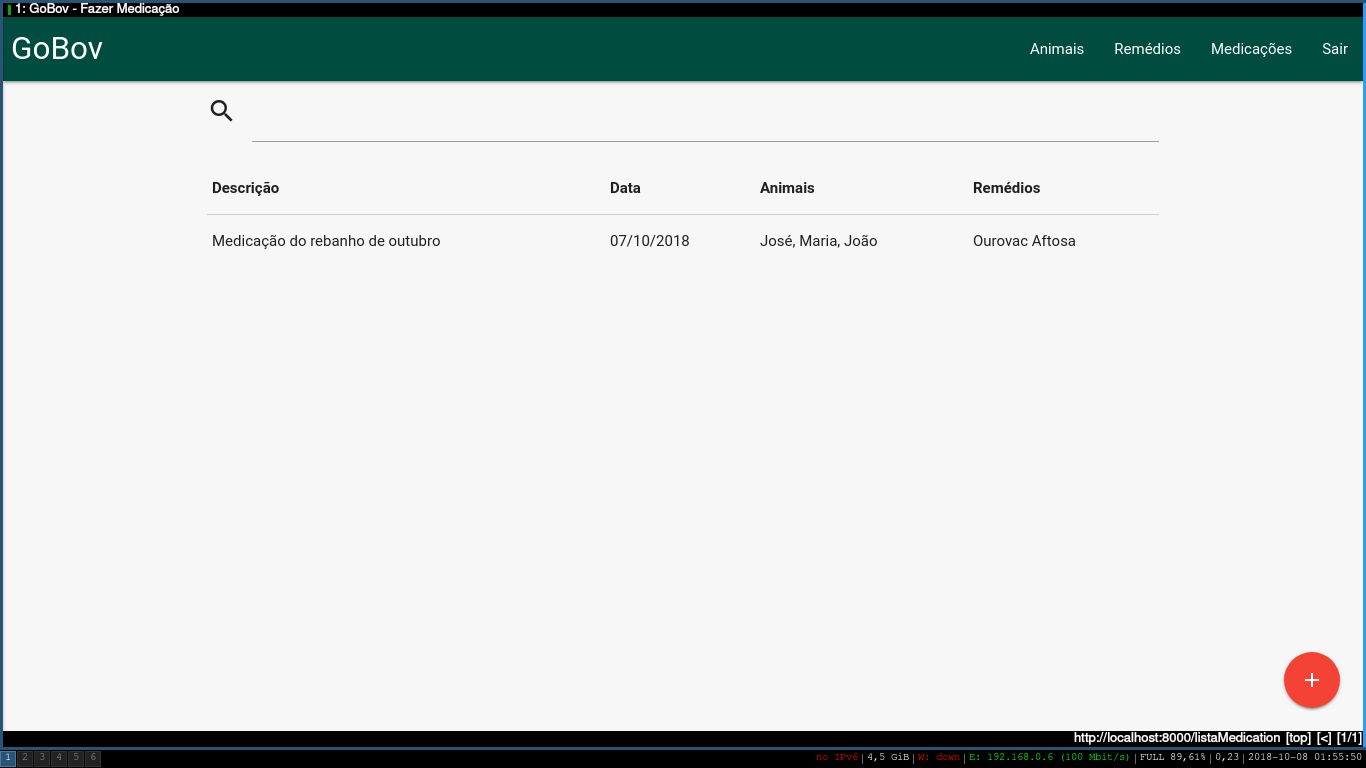
\includegraphics[width=\textwidth]{../img/prototipos/listaMedicacao.png}

		Fonte: Autoria própria.
	\end{center}
\end{figure}

\item IV008

A figura 12 é a página de adicionar medicação.
\begin{figure}[H]
	\begin{center}
		\caption{Página de adicionar medicação}
		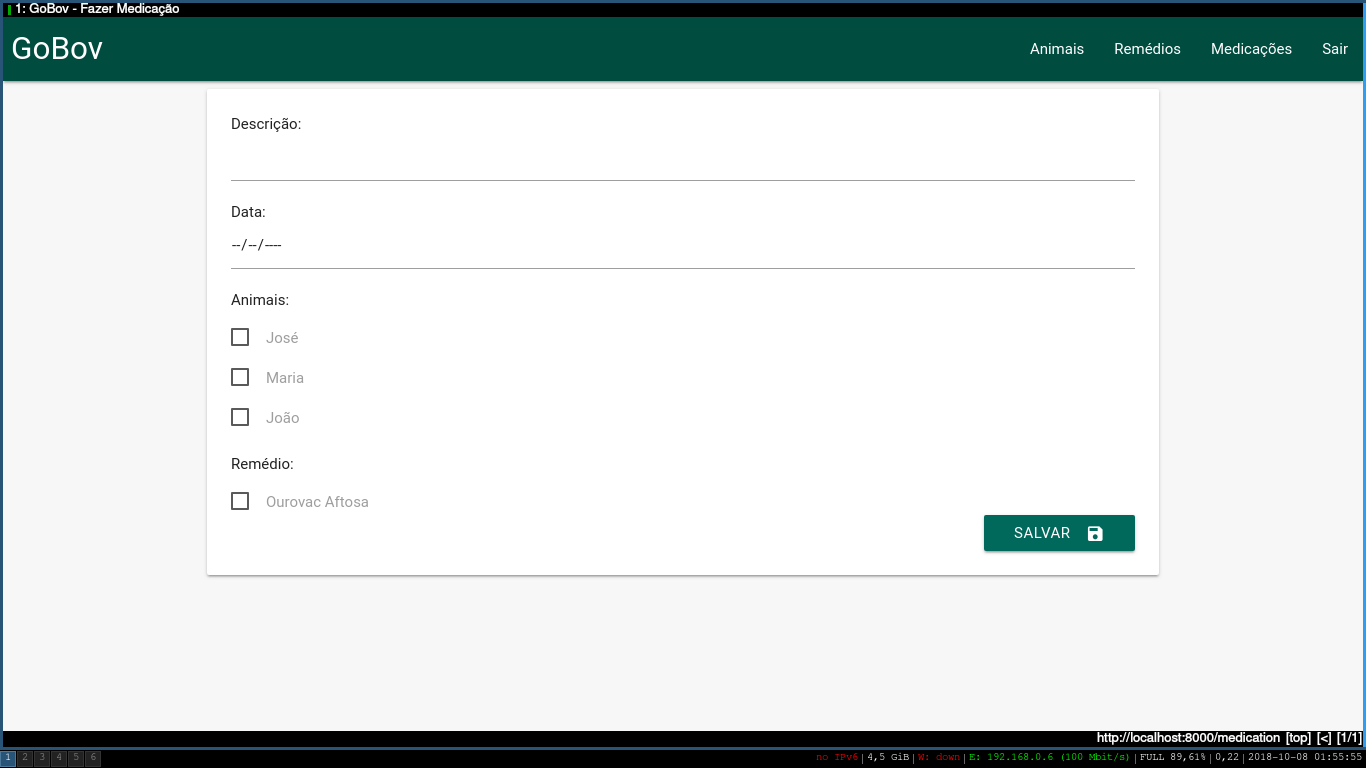
\includegraphics[width=\textwidth]{../img/prototipos/addMedicacao.png}

		Fonte: Autoria própria.
	\end{center}
\end{figure}

\item IV009

A figura 13 é a página de perfil do animal. Nela, o usuário pode editar, consultar detalhes, gerenciar uma pesagem do animal ou consultar relatórios individuais do animal.
\begin{figure}[H]
	\begin{center}
		\caption{Página de perfil do animal}
		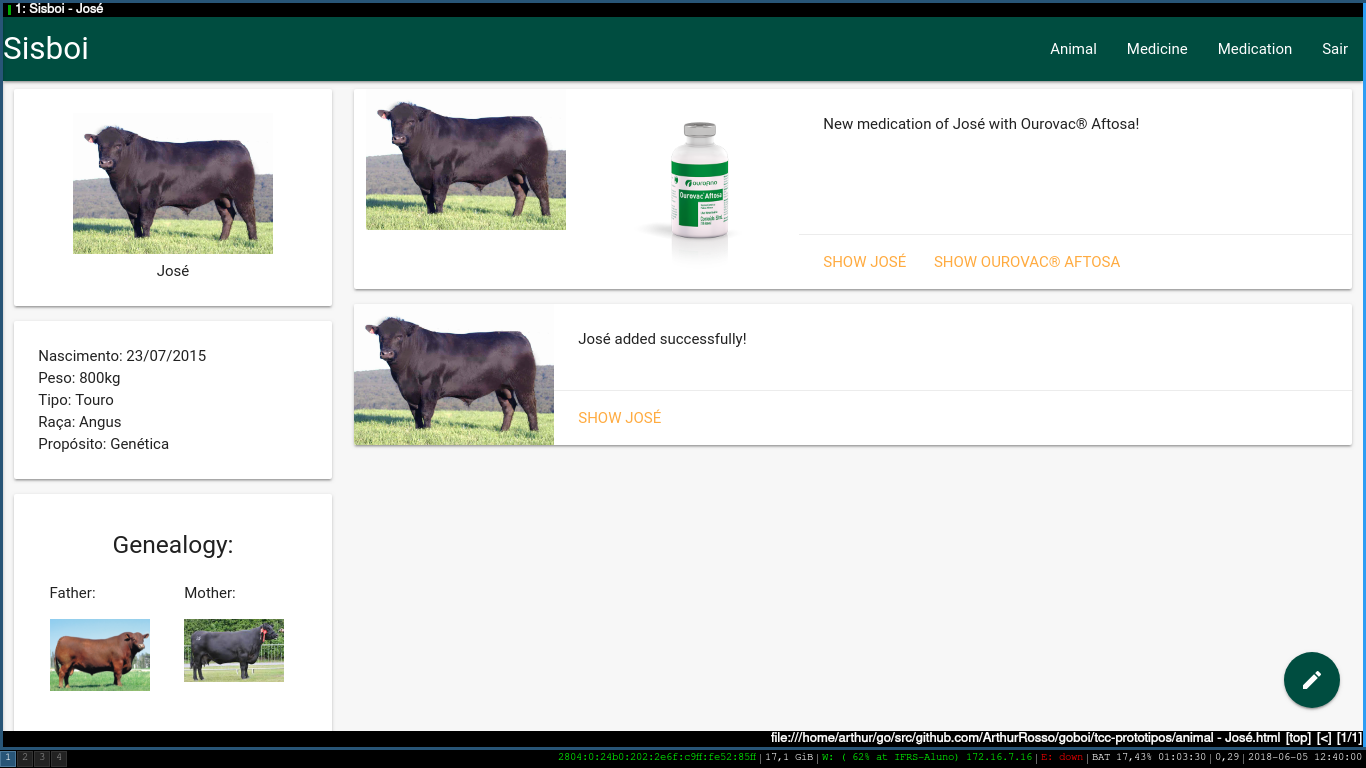
\includegraphics[width=\textwidth]{../img/prototipos/perfil.png}

		Fonte: Autoria própria.
	\end{center}
\end{figure}


\item IV010

A figura 14 é a página de edição do animal. Nela o usuário pode editar as informações básicas do animal.
\begin{figure}[]
	\begin{center}
		\caption{Página de edição do animal}
		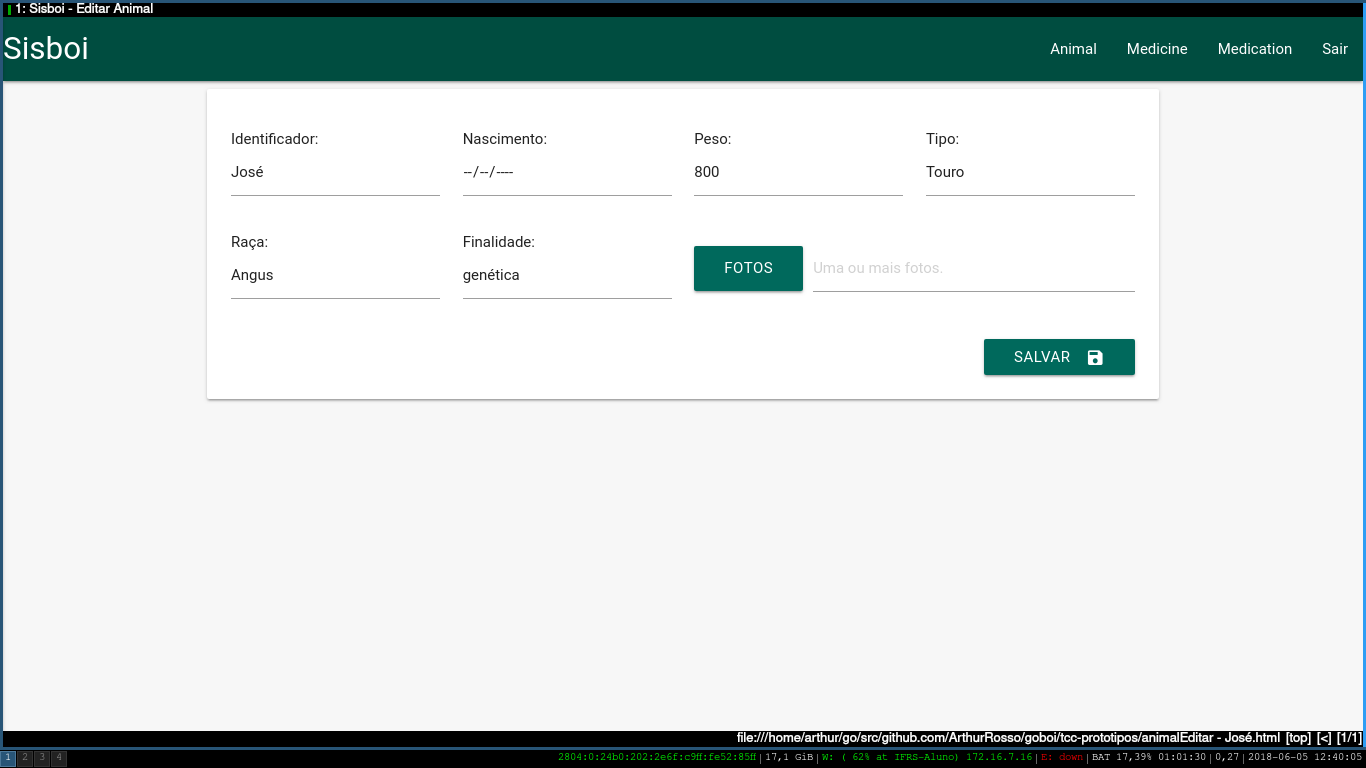
\includegraphics[width=\textwidth]{../img/prototipos/editar.png}

		Fonte: Autoria própria.
	\end{center}
\end{figure}

\newpage
\item IV011

A figura 15 é a página de pesagem. Nela o usuário pode gerenciar o peso de um animal.
\begin{figure}[H]
	\begin{center}
		\caption{Página de pesagem do animal}
		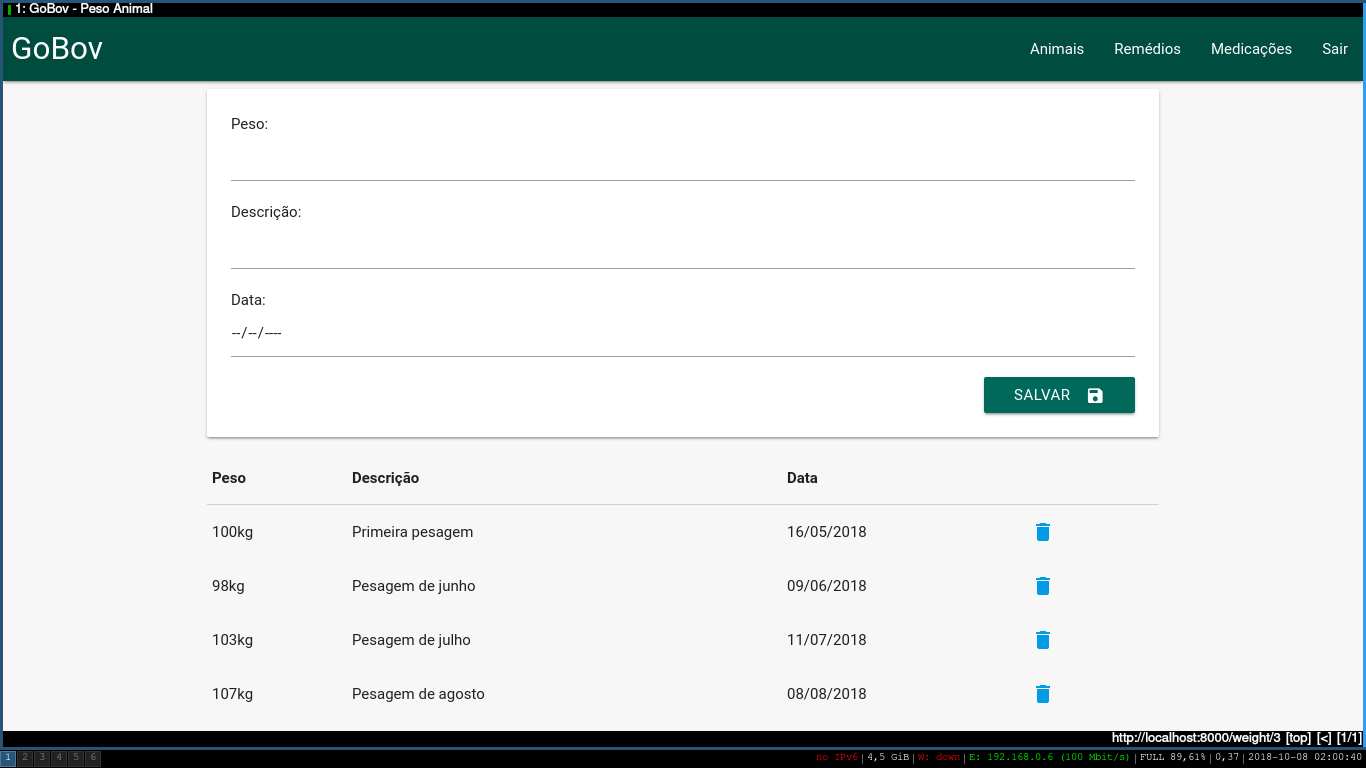
\includegraphics[width=\textwidth]{../img/prototipos/addPeso.png}

		Fonte: Autoria própria.
	\end{center}
\end{figure}

\item IV012

A figura 16 é a página de relatórios individuais do animal.
\begin{figure}[H]
	\begin{center}
		\caption{Página de pesagem do animal}
		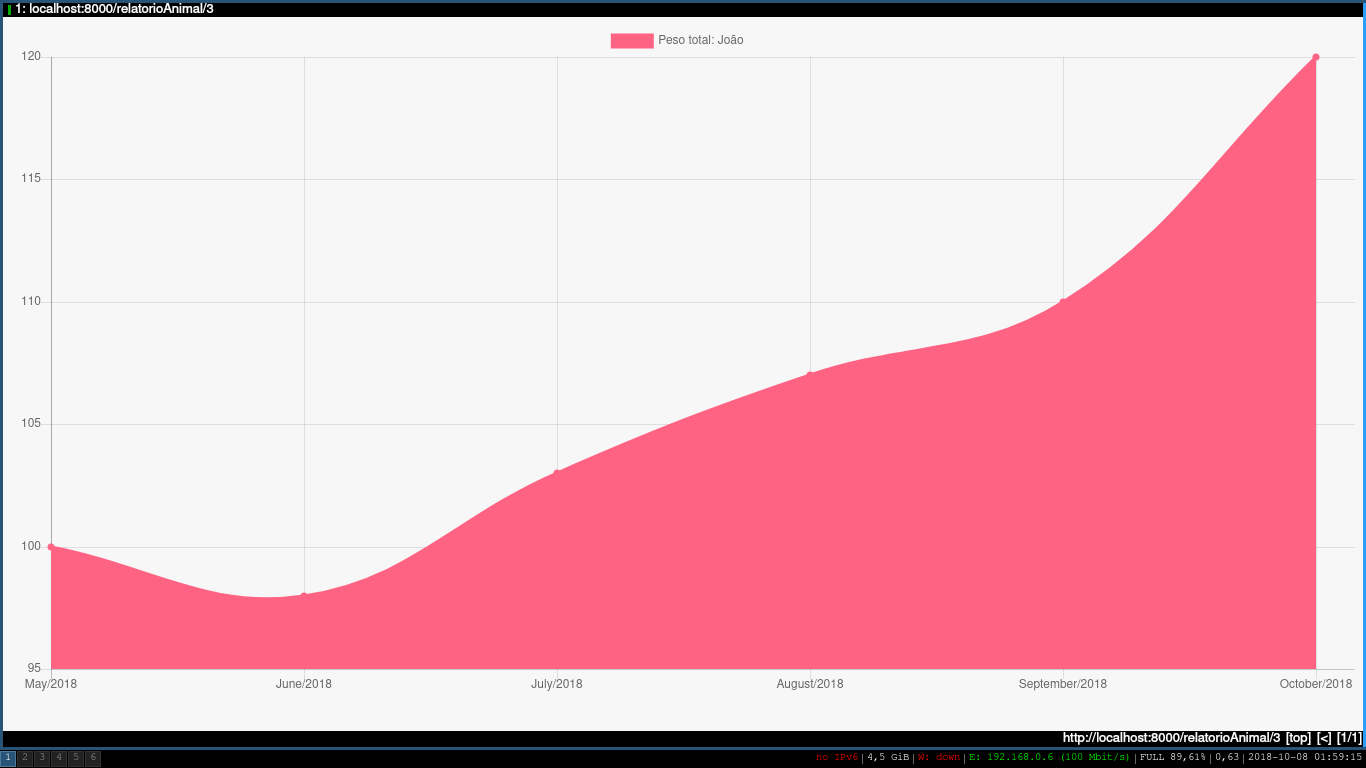
\includegraphics[width=\textwidth]{../img/prototipos/relatorio.png}

		Fonte: Autoria própria.
	\end{center}
\end{figure}

\end{itemize}

\section{MODELO ENTIDADE RELACIONAMENTO}

O diagrama a seguir mostra a abstração do banco de dados representando a relação do animal
com o usuário, com a foto, com o peso, com o propósito, com a raça, com o tipo, e com a remédio,
na qual é chamada de medicação. Por sua vez, o remédio também tem uma relação além da
medicação, que é o tipo.

\begin{figure}[H]
	\begin{center}
		\caption{Modelo ER}
		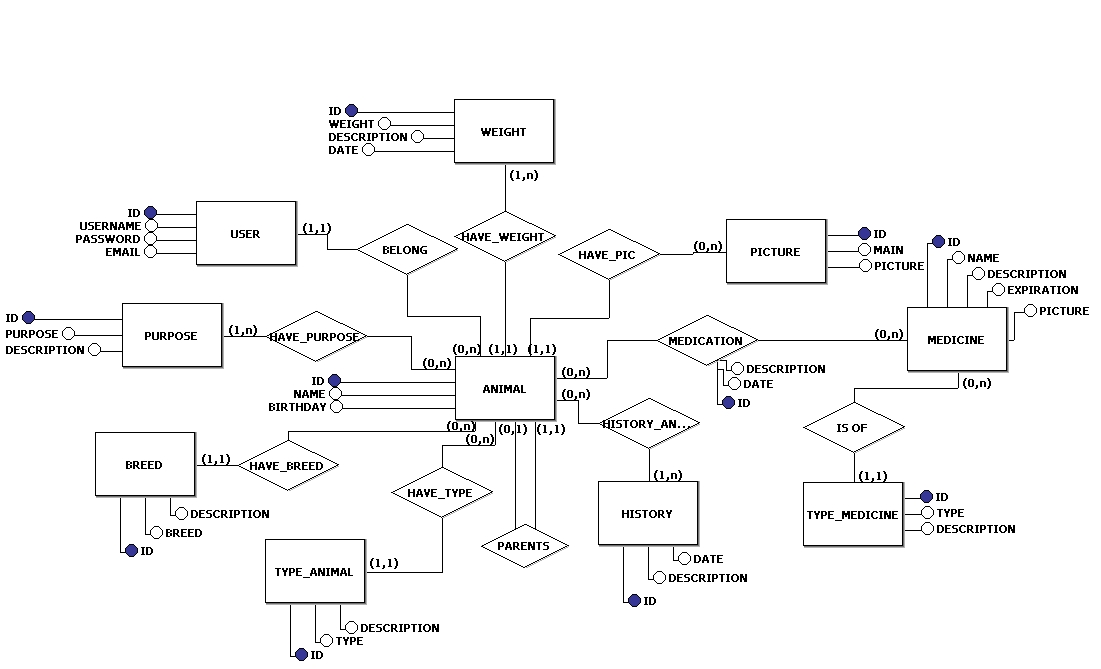
\includegraphics[width=\textwidth]{../img/erdoboi.jpg}

		Fonte: Autoria própria.
	\end{center}
\end{figure}
